\documentclass[12pt,twocolumn]{article}
\usepackage[utf8]{inputenc}
\usepackage[english]{babel}
\usepackage[table,xcdraw]{xcolor}
\usepackage{physics}
\usepackage{fancyhdr}
\usepackage{geometry}
\usepackage{natbib}
\usepackage{graphicx}
\usepackage{float}
\usepackage{wrapfig}
%\usepackage{caption}
\usepackage[justification=centering]{caption}
\usepackage{subcaption}
\usepackage{gensymb}
\usepackage[export]{adjustbox}
\usepackage{hyperref}
\geometry{margin = 20mm}
\usepackage{mathtools}
\usepackage{amsmath}
\usepackage{indentfirst}
\usepackage{xurl}
\usepackage{t1enc}
\usepackage{setspace}


\title{Simulating detectors with Geant4 final report}
\author{Scientific Modeling Computer Laboratory\\Bendegúz Borkovits T7UR9P\\Supervisor: Ákos Horváth\\Consultant: Balázs Pál}
\date{May 2022}


\begin{document}

\maketitle

\section{Introduction}

Geant4 is a software developed at CERN. Its main purpose is to allow the user to create virtual detectors to simulate and visualize the interaction of particles with each other and with the defined detector. The software provides a large variety in parameters for the simulations such as parameters that define the geometry of a detector and its material properties, the laws of physics that will be enabled in the proximity of said detector and many more.

The long-term aim of the project was to model the NEBULA detector of the SAMURAI Beam line. My task at first, consisted of following tutorials \cite{youtube} and the documentation \cite{geant} of the software to be able to grasp the knowledge on how a simulation in Geant4 could be created. To learn the steps of programming a simulation, I have followed a series of tutorial lectures that aimed toward creating a program that was centred around the appearance of Cherenkov radiation and detecting the resulting optical photons in the process. Then, I received a simulation of NEBULA by Balázs Pál and started to work with said program. I projected a beam on neutrons onto the detector, compared outputs yielded by different physics lists and did some analysis on the energy and particle data of the simulation.

\section{Building a simulation}

A simulation in Geant4 is a Cmake project, therefore, naturally one needs to start building it by defining its Cmake properties. Geant4 allows support for tools and environments such as Qt5 and Python, it also offers a multi-threading mode, though in this project everything was done in single-threading mode in order not to run into a few problems regarding multi-threading and its effect on the simulations. Geant4 offers support for various operating systems such as Ubuntu and Windows. It should be noted that the Windows version runs considerably slower than its Linux counterpart, therefore in this project Ubuntu 18.04 was used as the environment. Said operating system was used as a virtual machine, set up in the Oracle VM VirtualBox application. Although, 18.04 is not the newest version of Ubuntu, it seemed to be more stable when started from VirtualBox than the newer versions.

After setting up the environment and the respective Cmake files, I started to define structure of the simulation. To make the project seem more organized, one should divide the program into individual parts according to their respective purpose. Firstly, the main function of the simulation was defined and contained int the file \emph{sim.cc}. Said function consists of the executive commands and some refinement commands for the visualization. Then, defining the geometry should be the next part in the process. This step of the simulation is contained in the files \emph{construction.cc} and \emph{construction.hh}. First, one should declare the shape and size of the world itself. In this case, the world volume is simply a box with the width, length and height of one meter. The logical and physical parameters of the world consist of it having air inside of it and having the origin of the coordinate system in its centre. After that, one should create a desired detector. The parameters of said detector are made up by its geometry and material properties. In Geant4, one is able to create complex molecules by defining and combining simpler molecules. To this end, I built up silicon-dioxide, water and carbon molecules to combine them into an aerogel detector that consist of the following percentages of the previously mentioned molecules: 62.6\%, 37.4\% and 0.1\%. Finally, I defined the shape of the detector as a smaller box with considerably smaller length than width and height and placed it inside the world volume. It should be noted that the different sizes of the detector always need to be smaller than that of the world volume.

\begin{figure}[H]
    \centering
    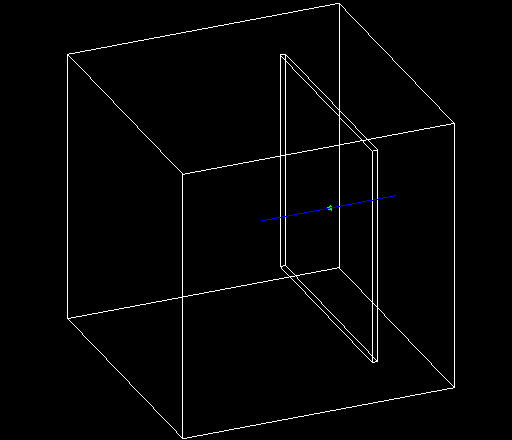
\includegraphics[scale=0.64]{detector_volume.png}
    \caption{The box shaped detector contained within the world volume. The blue line indicates the defined proton and the green line indicates the optical photons that were produced via Cherenkov radiation. Sometimes red lines also appear, indicating the presence of $\beta$-electrons.}
    \label{fig:basic}
\end{figure}

As a next step, one should generate a few particles. In this project the G4ParticleGun class was used as a generator. To test whether this method works, I generated a proton with a Z-directional momentum of 100 GeV that goes through the centre of the detector. The properties of said proton were defined in files \emph{generator.cc} and \emph{generator.hh}. For computing purposes, one should define an action manager that manages the process of particle generating. This part of the simulation is included in \emph{action.cc} and \emph{action.hh}. The mentioned files can be viewed on my Github page. \cite{borbende}

The final step in completing the simulation is creating a suitable physics list, in this case enabling the occurrence of optical photons and the existence of electromagnetic interaction. The code of this step is located in files \emph{physics.cc} and \emph{physics.hh}. The result is showcased on Figure 1. The proton collides and goes through the detector, while optical photons are produced upon entry as Cherenkov radiation.

\section{Detecting photons}

In order to inquire information about the optical photons, they need to propagate through the aerogel detector and collide with a wall made of small sensitive detectors. To that end, one needs to define the refractive indices of the aerogel detector and the world volume separately. Then, one should include the properties of the photo-sensitive detectors into the simulation. The material properties and geometry were defined in the file \emph{construction.cc}. Essentially, I created a wall that has a small detector for every segment and each of these can detect an incoming photon. Finally, one needs to precisely tell the program, what kind of information one would like to gain. As an easier example, I have asked information about the positions where the photons enter the wall of sensitive detectors. The resulting data consisted of the position of the side of the detector that was closer to the aerogel box. The declarations of this information can bee seen in files \emph{detector.cc} and \emph{detector.hh}.

Saving the output of a Geant4 simulation is relatively straight forward. One needs to create several columns to separate the different datasets and fill them with the yielded results. There are four file formats one can work with regarding Geant4. These are the following: ROOT, CSV, XML and HBOOK. ROOT seems to be the favoured method for working with Geant4 and to that end, I have installed the ROOT software to test the accessibility of said format. In the end, working with CSV files turned out to be the more favourable option, as I was planning to evaluate my data using Python and the NumPy module provides user friendly methods to deal with CSV files. Saving the output requires the creation of a run manager that manages all the saving commands and works with the built-in library of the chosen file format, such as g4csv. The run manager was put into the files \emph{run.cc} and \emph{run.hh}.

\begin{figure}[H]
    \centering
    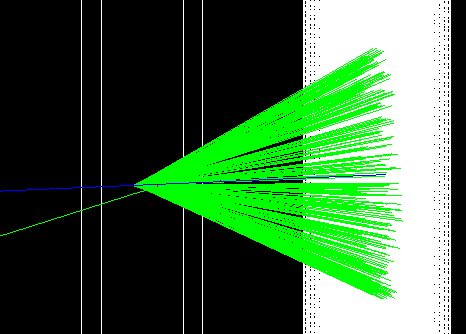
\includegraphics[scale=0.8]{sensitive_detectors.png}
    \caption{The proton (blue) produces the cone of photons (green) when going through the aerogel detector and the photons reach the sensitive detectors (white). The tiny red line indicates a $\beta$-electron. The one photon on the other side of the detector is some back scattering event that occurs with very low probability.}
    \label{fig:my_label}
\end{figure}

\section{Showcasing the output}

To plot the positions, where the photons entered the wall of detectors, I used matplotlib.pyplot in a Jupyter notebook. To generate data, I saved ten events of Cherenkov radiation caused by a proton, meaning that I ran the simulation ten separate times and stored the information yielded by each run in a single file. Then, I checked the distribution of the number of photons generated by each event. The result is showcased on Figure 3. It can be seen that each run generates almost the same number of photons with a mean of $308\pm17$ particles. Then, I plotted the XY-coordinates of each data point and checked whether or not the extraction of the results was successful by expecting a circle to be formed. The result can be seen on Figure 4.

\begin{figure}[H]
    \centering
    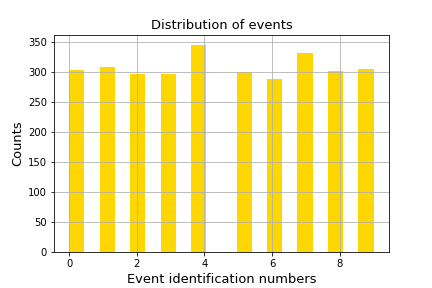
\includegraphics[scale=0.65]{histo.png}
    \caption{Showing the amount of photons generated by each individual run. They showcase a rather uniform distribution.}
    \label{fig:my_label}
\end{figure}
\begin{figure}[H]
    \centering
    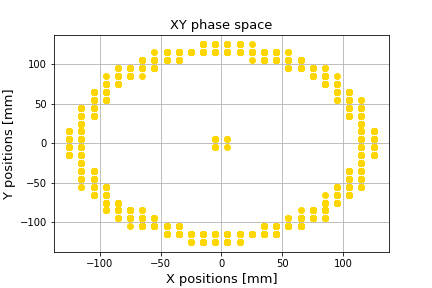
\includegraphics[scale=0.65]{xy_phase.png}
    \caption{Showcasing the positions of the photons upon entry to the sensitive detector wall on the XY-plane.}
    \label{fig:my_label}
\end{figure}

On Figure 4, one can indeed view the circular shape, however four data points were shown in the middle of the figure. This is once again due to the occurrence of some sort of low probability scattering event that places a photon in the run that it happens in the middle of the figure. The evidence that suggest this are the facts that the proton does not interact with the sensitive detectors and this happens only four times out of ten runs. The evaluation of the data can be found in file \emph{analysis.ipynb}. \cite{borbende}

\section{The NEBULA detector}

NEBULA itself is a plastic scintillator array with a large volume that is used to simulate and measure fast neutron events at the 100-300 MeV range that are emitted at forward directions in processes such as nuclear breakup. \cite{nebula} NEBULA is part of the SAMURAI beam line at the RIKEN RI Beam Factory in Wako, Japan, a heavy-ion research facility where the world's largest superconducting ring cyclotron is located. \cite{RI}

\begin{figure}[H]
    \centering
    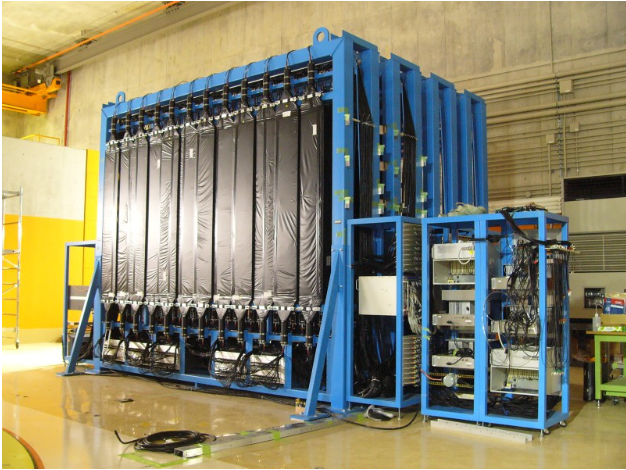
\includegraphics[scale = 0.65]{nebulakep.png}
    \caption{Showcasing the NEBULA detector at the RIKEN RI Beam Factory in Wako. \cite{nebula}}
\end{figure}

NEBULA contains neutron detectors (NEUT), charge-particle veto detectors (VETO) and these are separated into several modules that are made up of plastic scintillators (BC-408) and photomultiplier tubes (PMT) that are connected to the ends of the scintillators by light guides. The modules themselves are organized into a two-layer detector wall. Altogether, the wall consists of 120 NEUT and 48 VETO modules of which 24 are in reserve. \cite{nebula}

The team of scientists working with NEBULA created their own simulator of the detector. Smsimulator is a C++ program based on Geant4 that allows for the virtualization of NEBULA and is updated rather frequently. \cite{smsim} It offers a few services such as, simulating response to a single neutron, simulating trajectory of charged fragment in the SAMURAI magnet and a simulation for N-body neutron decay. The program uses ROOT libraries for visualisation. Due to these qualities, this simulation tool would be extremely useful. However, installing it is no easy feat as it requires numerous adjustments in the configuration files of ROOT and Geant4 and is also only compatible with a few specific versions of Geant4. Due to the earlier mentioned reasons, I have been unable to install and run smsimulator. After consulting with my supervisor, we opted to use the NEBULA simulation made by Balázs Pál, two years prior. \cite{masterdesky} However, after applying a few modifications and attempting to run said program, an error occurred that originates from the original simulation. The problem was since resolved but it took considerable time away from progress.

\section{The predefined parameters}

One two-layered wall of the NEBULA consists of sixty NEUT and twelve VETO modules of which, here only eighteen neutron detectors are modelled. \cite{nebula} To generate the required data, a neutron beam that consisted of one hundred particles with 100 MeV initial energy was projected onto the wall. This process is shown on Figure 6. After the beam interacts with the various modules in the wall, multiple events occur like ionization, elastic scattering, back scattering and so forth. Numerous new particles are detected in the process like protons, deuterons, or photons. Due to this, a problem has arisen with the visualization. Although, Geant4 provides an excellent visualization tool for our experiments, even it has its limit in distinguishing all the different types of by-product particles. There are some methods to make the output more pleasing to the eye, however in this case, it might not work due to the large number of particle types.

\begin{figure}[H]
    \centering
    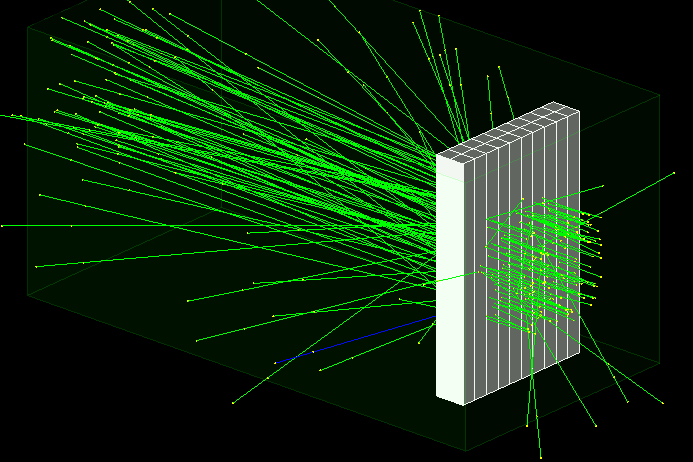
\includegraphics[scale = 0.5]{qbbc_neutbeam.png}
    \caption{Showcasing the trajectory of the neutron beam.}
    \label{fig:my_label}
\end{figure}

One might ask, what kind of physics lists would the measurement of neutrons require. For this purpose, Geant4 offers a great deal of choices. \cite{geant} This is rather joyous news, since it is our task to examine the output of the simulation using various physics lists. The lists chosen for this simulation are the following. Four different lists of the QGSP physics list library that stands for Quark Gluon String Physics and works around said model. These are BERT\_HP that uses the Geant4 Bertini Cascade, BIC\_HP that uses the Binary light Ion Cascade, INCLXX that revolves around the Liege Intranuclear Cascade model, and INCLXX\_HP that is similar to the earlier mentioned one but also includes the data driven high precision neutron package (HP). \cite{geant}

\section{Analysis and results}
After running the simulation once for every physics list, we obtained the figures that are shown in the appendix of this document. The relative number of particles means the number of particles rendered to a given category in the histogram, like number of protons or number of particles detected by the fourteenth NEUT module.

When we categorize the number of particles by their type, it is shown on Figure 7 that the protons generated by the interaction between the beam and the detector is the highest or is almost equal to the number of neutrons present. This behaviour reappears on all five subplots. It is because of these results, that we show no surprise when realizing upon looking at Figure 8 that the dominant particle generating processes during the simulation were hadronic processes. Then, when taking a look at the number of particles detected by the different modules, it is shown on Figure 9 that the corners on the wall, that consist of Counter1, 2, 16 and 17 detected the least of them as expected.

Upon measuring and plotting the deposited energy, I sorted the values in descending order to have a better view of the situation. The protons were shown to have the largest amount of deposited energy on Figure 10. Unsurprisingly, the already determined most dominant hadronic ionization process was detected to be dominant in energy as well, as it was showcased on Figure 11. Finally on Figure 12, we noticed that there are quite a few differences between the order of Counters on the different subplots. However, this is only due to the fact that the difference in energy between many Counters is negligible and thus prone to change with randomness during each run. Also, it does not come as a surprise that the energy deposited to the world volumes is significantly less than those deposited to the modules.

Since, it has been determined that protons were the most prominent by-products of the experiment, my next task revolved around them. This task consisted of measuring the total energy deposited by each individual proton into the Counters they came into contact with during their respective events. When showcasing the energy, one should take into account the detector efficiency in such a way, that many energy values during the measurement are depicted as 0 or close to that. For this reason, one should display hits with energy higher than a value that is well-between 0 and an acceptable amount of energy detected. Let this number be 0.01 MeV in this experiment. A more serious problem arises with the fact that each hit of the same particle is counted as a separate particle. For this reason, one must include the TrackID or even EventID of the particles into the simulation. The TrackID marks each individual particle and tracks them throughout the whole run of the simulation thus, the previously separate particles will count as the hits of a single particle. The EventID is not important in this case, as it only serves to group a neutron and all its by-products by a single ID number.

After including the previously mentioned changes into the program, I ran it five times to see how randomness affects the results. In the file proton.ipynb, a matrix was created, called the TrackID by Volume matrix that has the TrackID of the individual protons as rows and the NEUT modules as columns, while the values of the matrix are the summed energy values. I plotted the individual columns of the matrix and repeated this process for each run. The yielded plots can be viewed on Figures 13-17. As it can be seen, there will almost always be some higher energy protons, while the majority of the particles deposit very low or next to no energy. The latter is due to the fact, that each proton only interacts with a given number of counters and the rest of the interactions were dumped by the detector efficiency. The randomness that affects the results changes the number of protons, the amount of deposited energy and the number of volumes one can take into account after accounting for detector efficiency. All in all, the results can sometimes differ drastically.

\section{Discussion}

While working on the project, I have come to the conclusion that Geant4 is an incredibly difficult tool to use, as coding and debugging in it can be a nightmare even when following strict guidelines.

In the end, the majority of my tasks was accomplished, I have learned how to create a simulation in Geant4 while working on the Cherenkov radiation program. Then, I learned how to save and analyse data produced by Geant4. Finally, I conducted comprehensive analysis on the NEBULA simulation. The only step, I was not able to achieve, was to completely automatize the simulation. I have also encountered numerous issues while working on the project that delayed my progress sometimes by a few weeks even. However, all of these issues have been resolved.

\section*{Acknowledgement}
A word of thanks is in order for the invaluable help provided by both Ákos Horváth and Balázs Pál.


\bibliographystyle{plain}
\bibliography{references.bib}


\onecolumn
\section*{Appendix}

\begin{figure}[H]
    \centering
    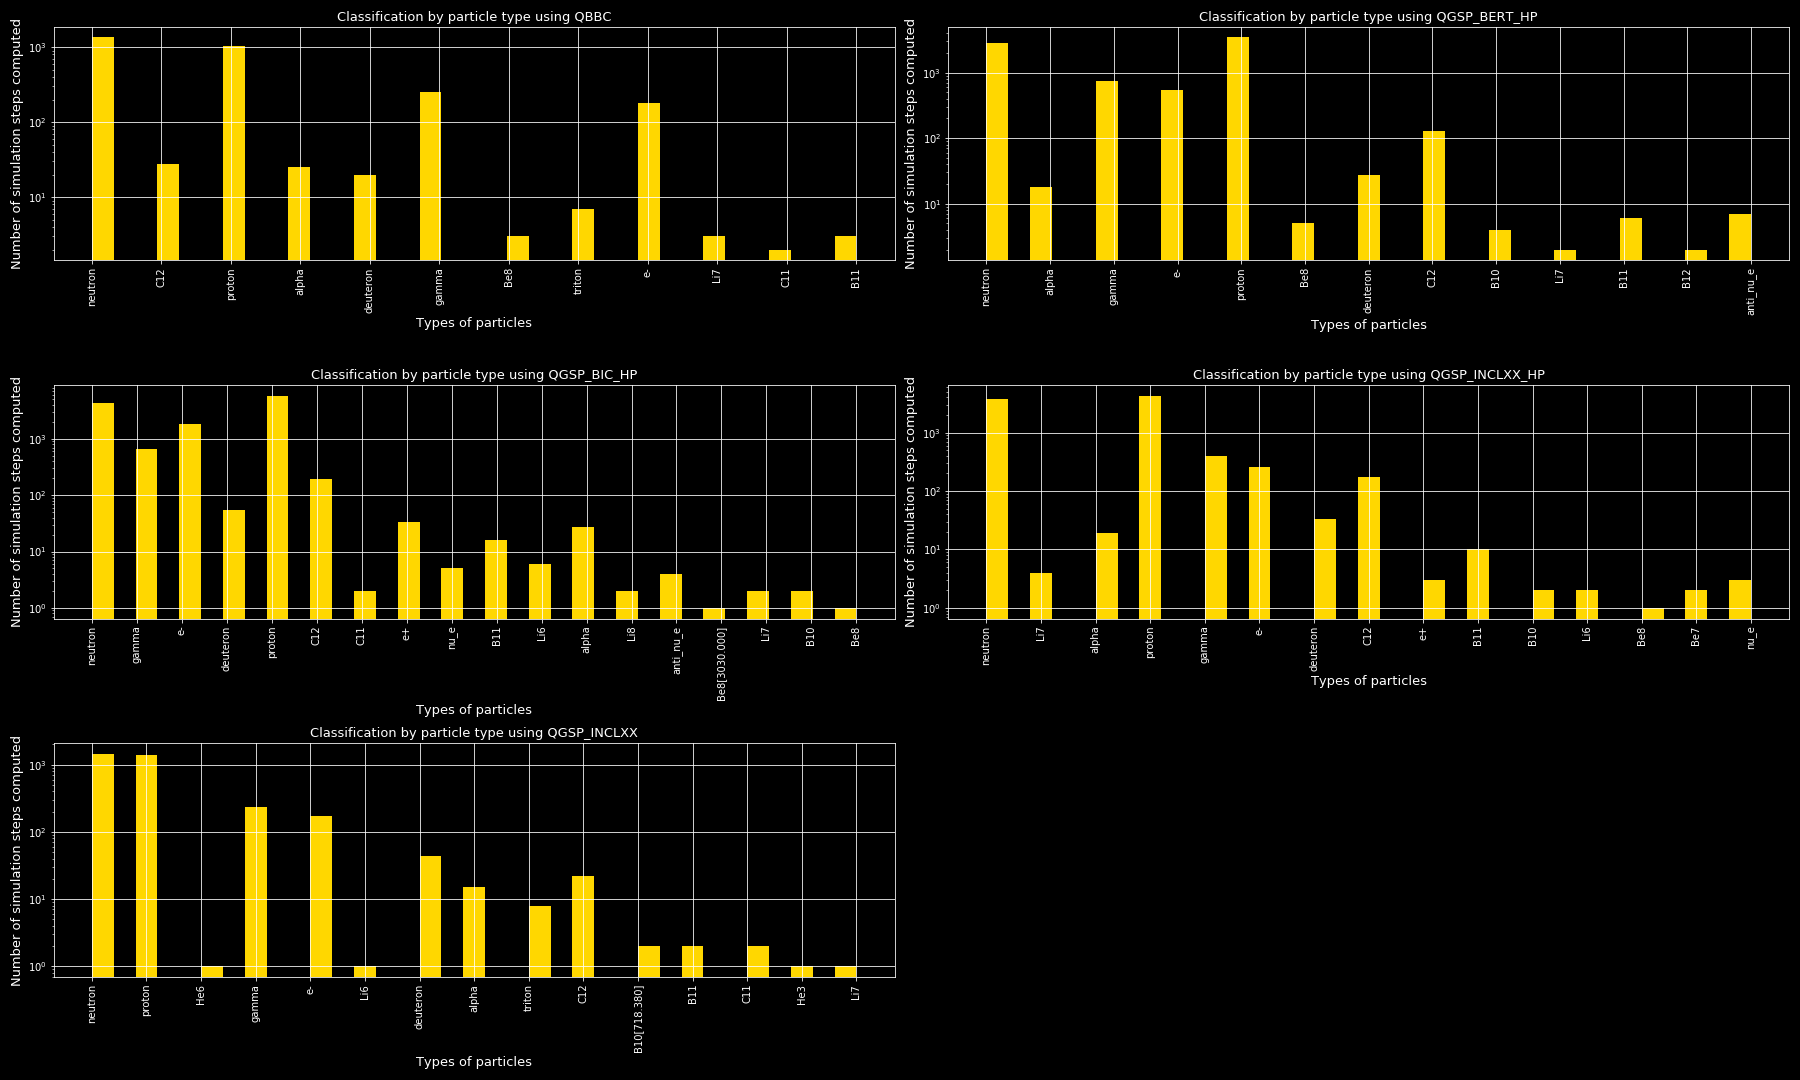
\includegraphics[scale = 0.25]{numparticles.png}
    \caption{Summing the relative number of particles by their types.}
    \label{fig:my_label}
\end{figure}

\begin{figure}[H]
    \centering
    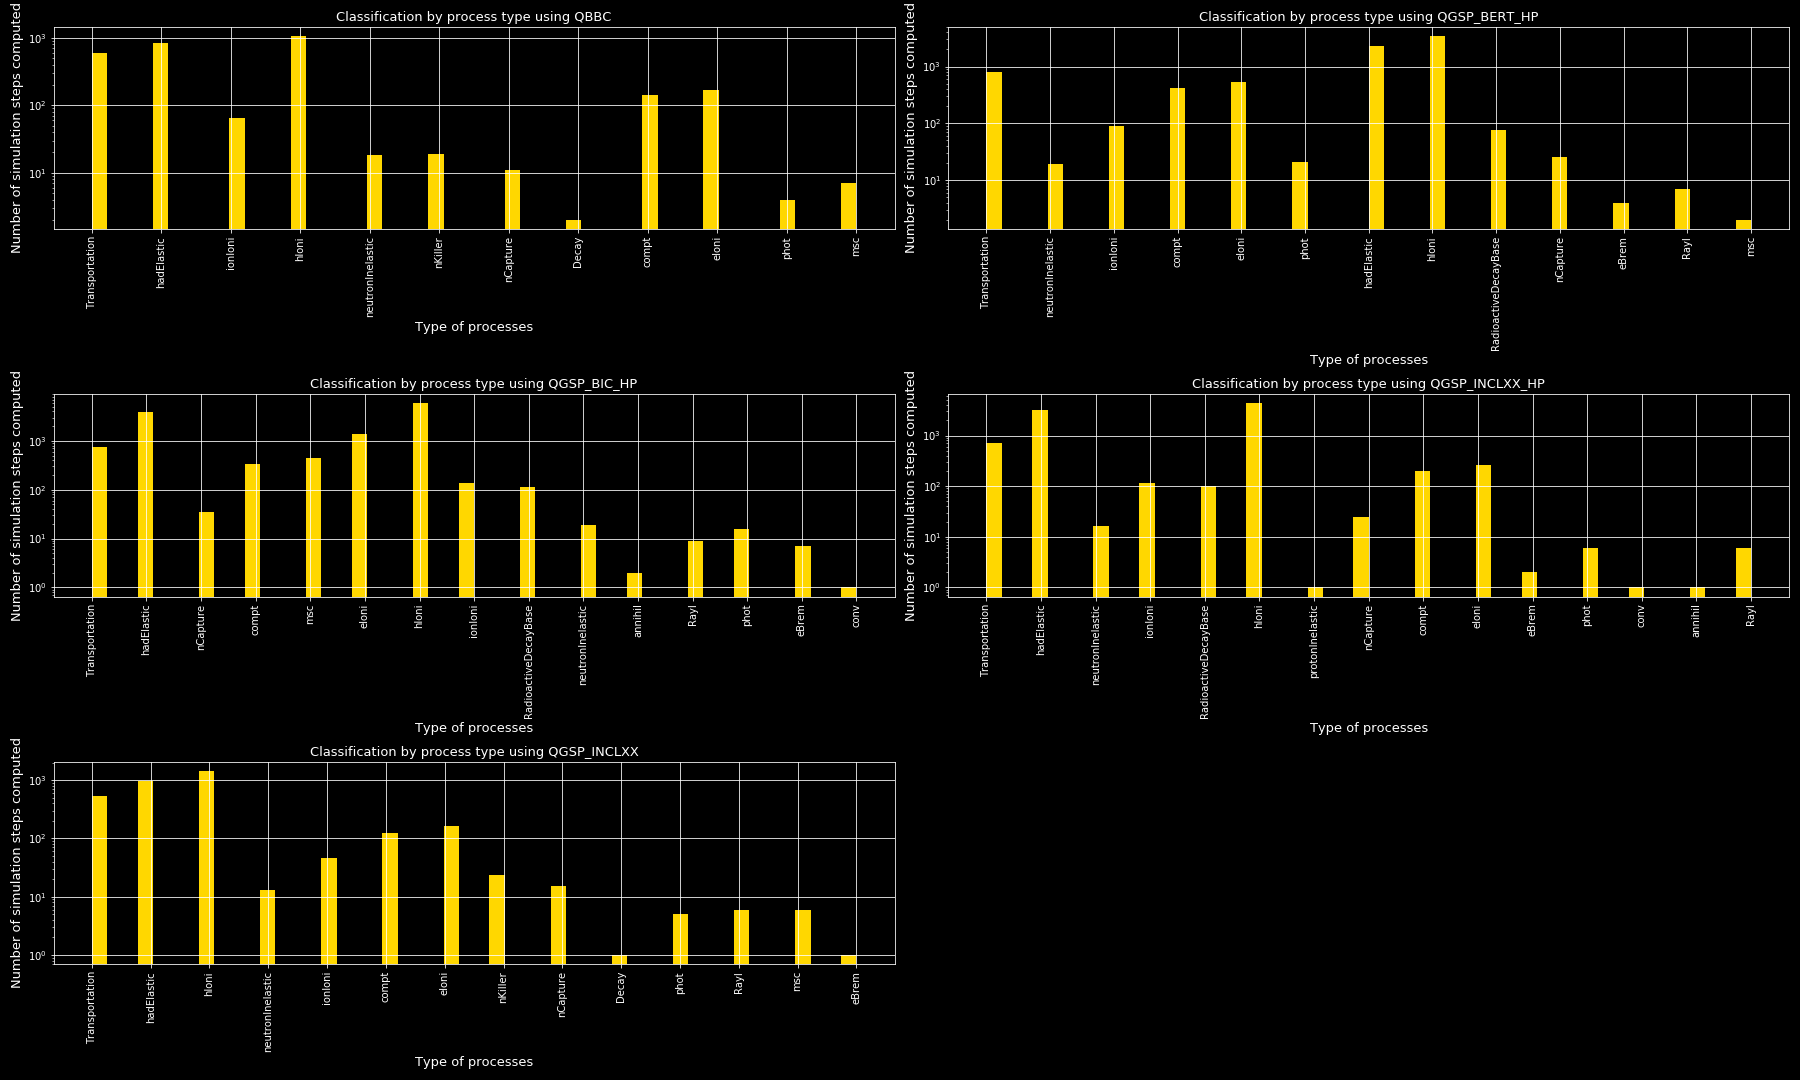
\includegraphics[scale = 0.25]{numprocess.png}
    \caption{Summing the relative number of particles by the processes that generated them.}
    \label{fig:my_label}
\end{figure}

\begin{figure}[H]
    \centering
    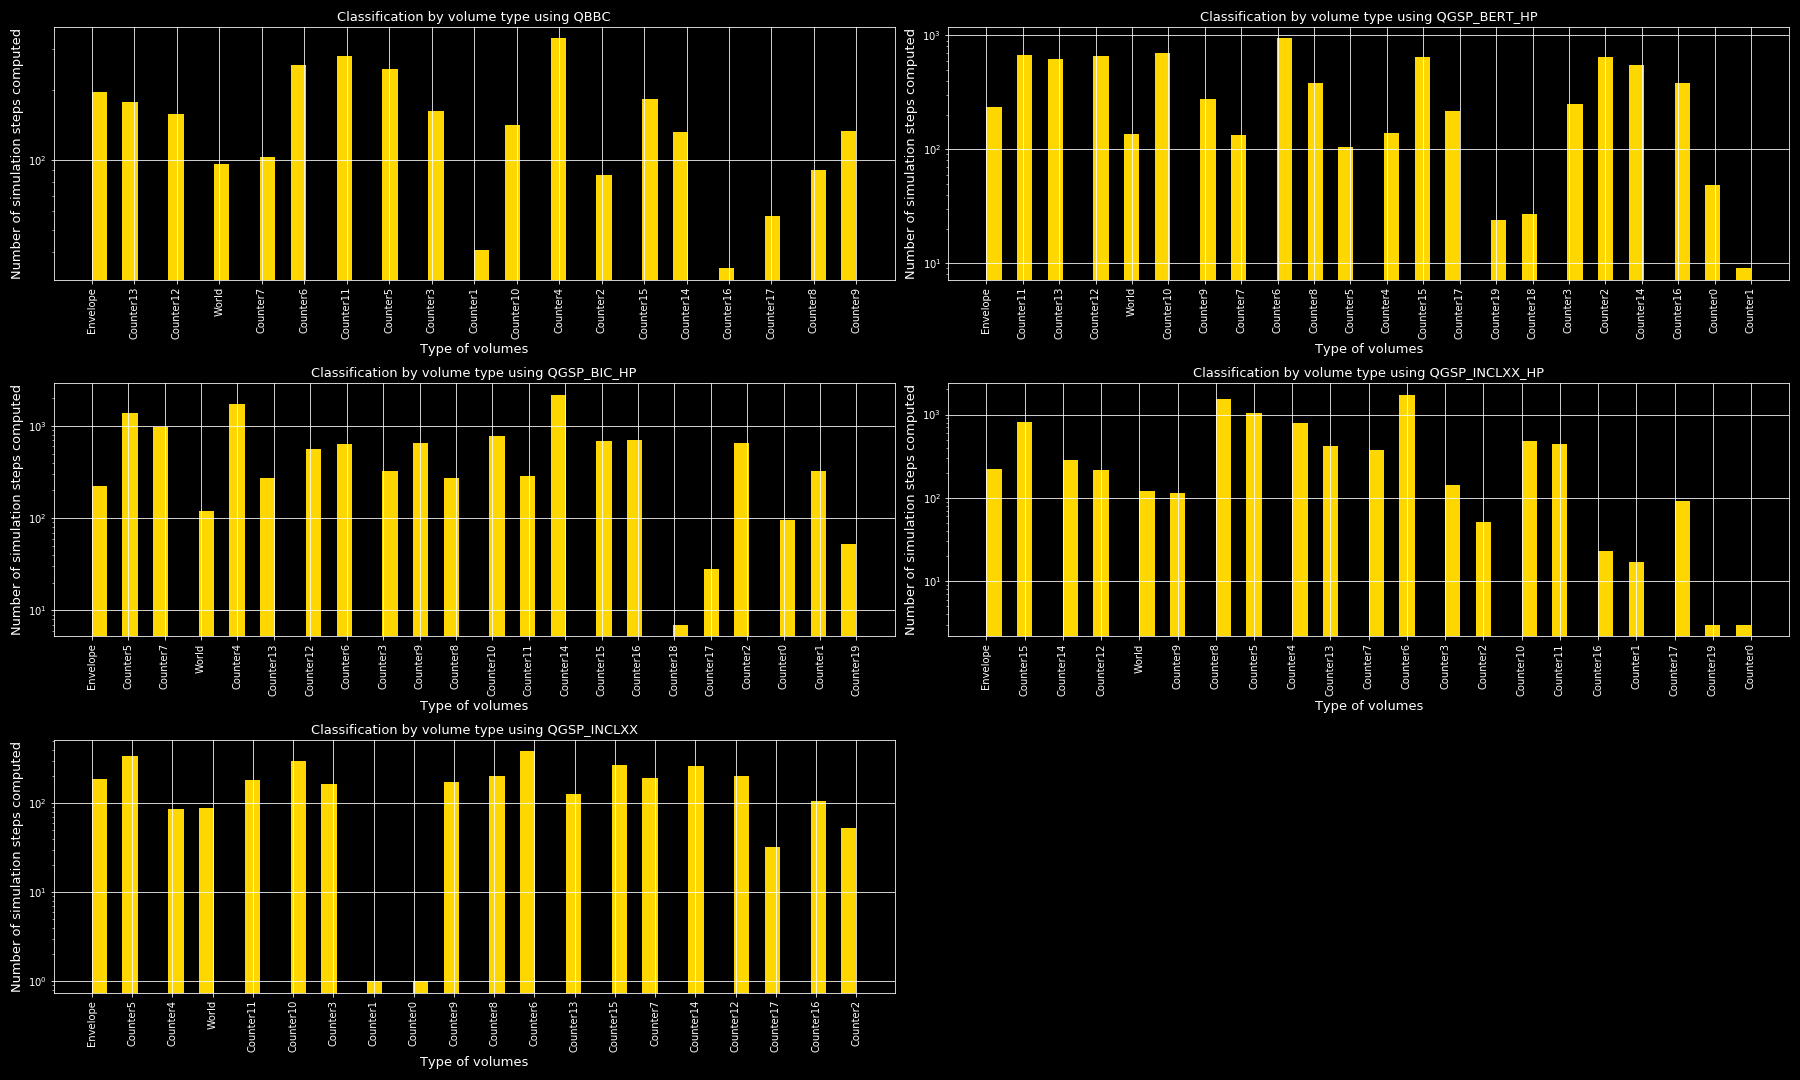
\includegraphics[scale = 0.25]{numvolumes.png}
    \caption{Summing the relative number of particles by the volumes they were detected in.}
    \label{fig:my_label}
\end{figure}

\begin{figure}[H]
    \centering
    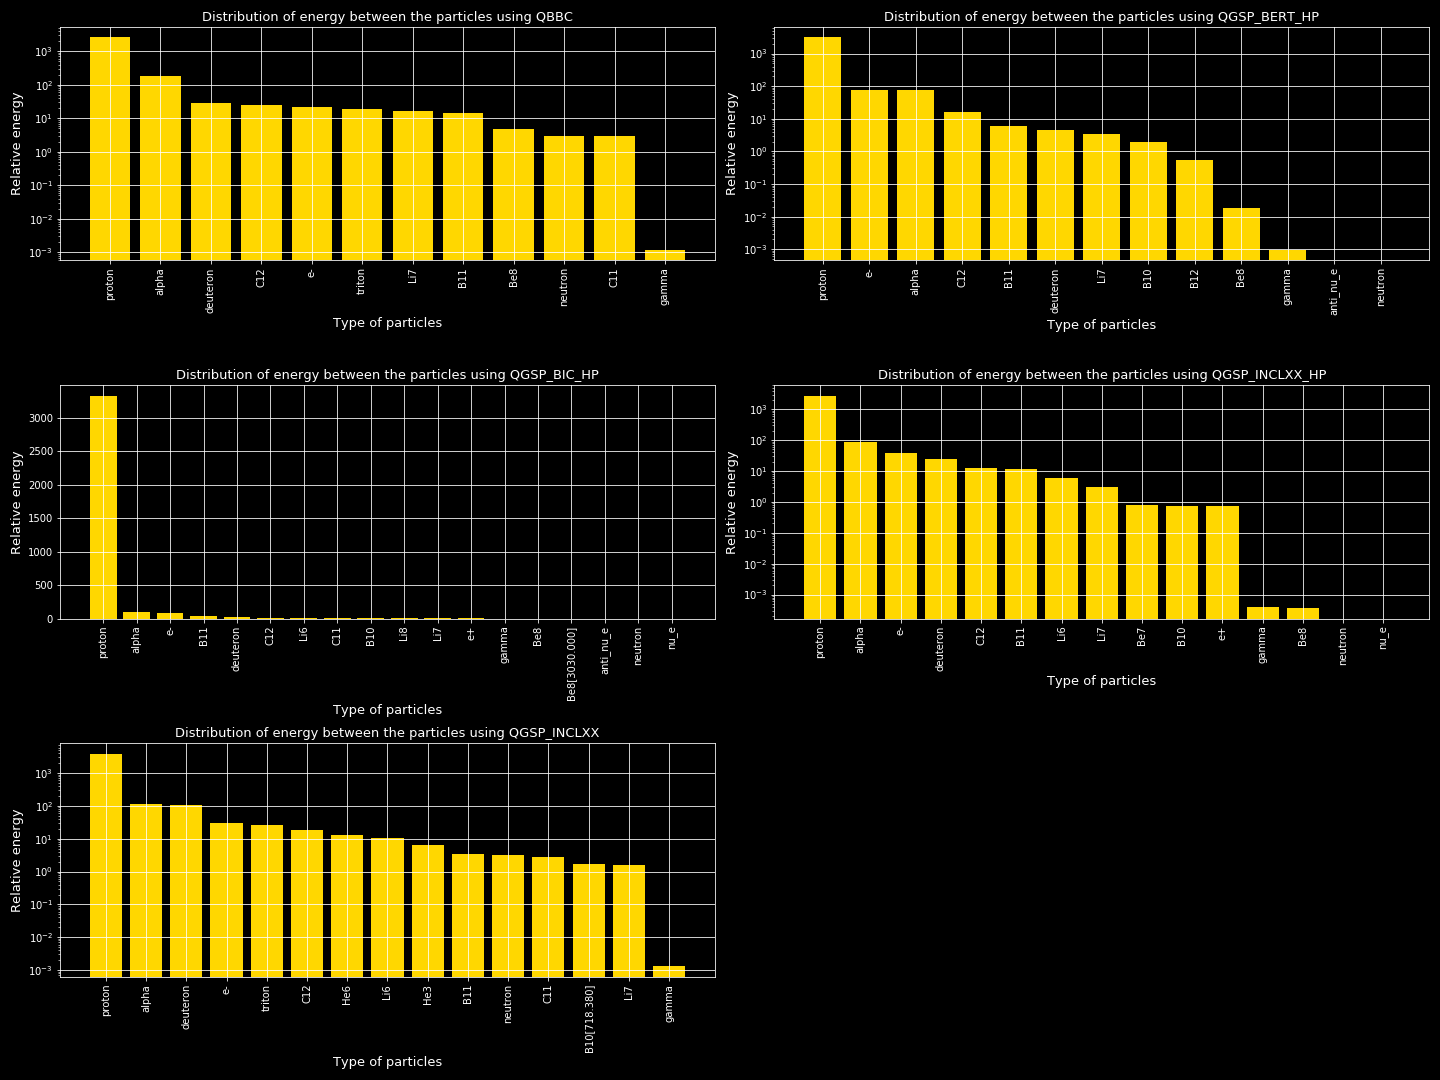
\includegraphics[scale = 0.30]{enpart.png}
    \caption{Summing the relative energy distributed among the particles by particle type. The log scale of the third subplot was bugged.}
    \label{fig:my_label}
\end{figure}

\begin{figure}[H]
    \centering
    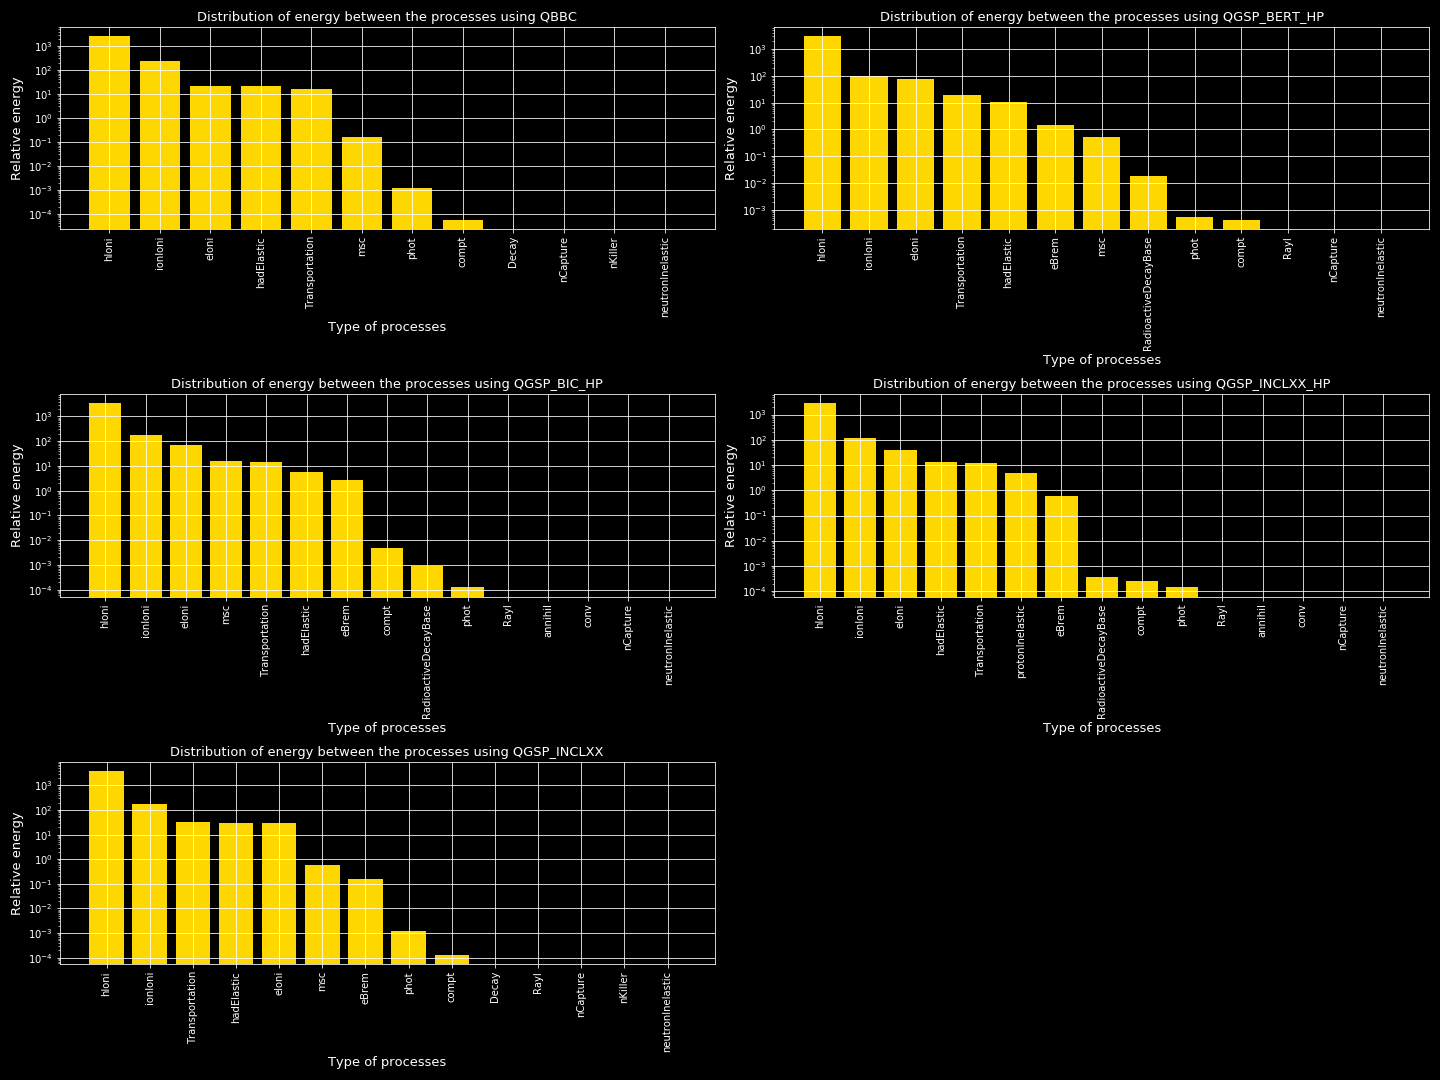
\includegraphics[scale = 0.28]{enproc.png}
    \caption{Summing the relative energy distributed among the particles by generating process.}
    \label{fig:my_label}
\end{figure}

\begin{figure}[H]
    \centering
    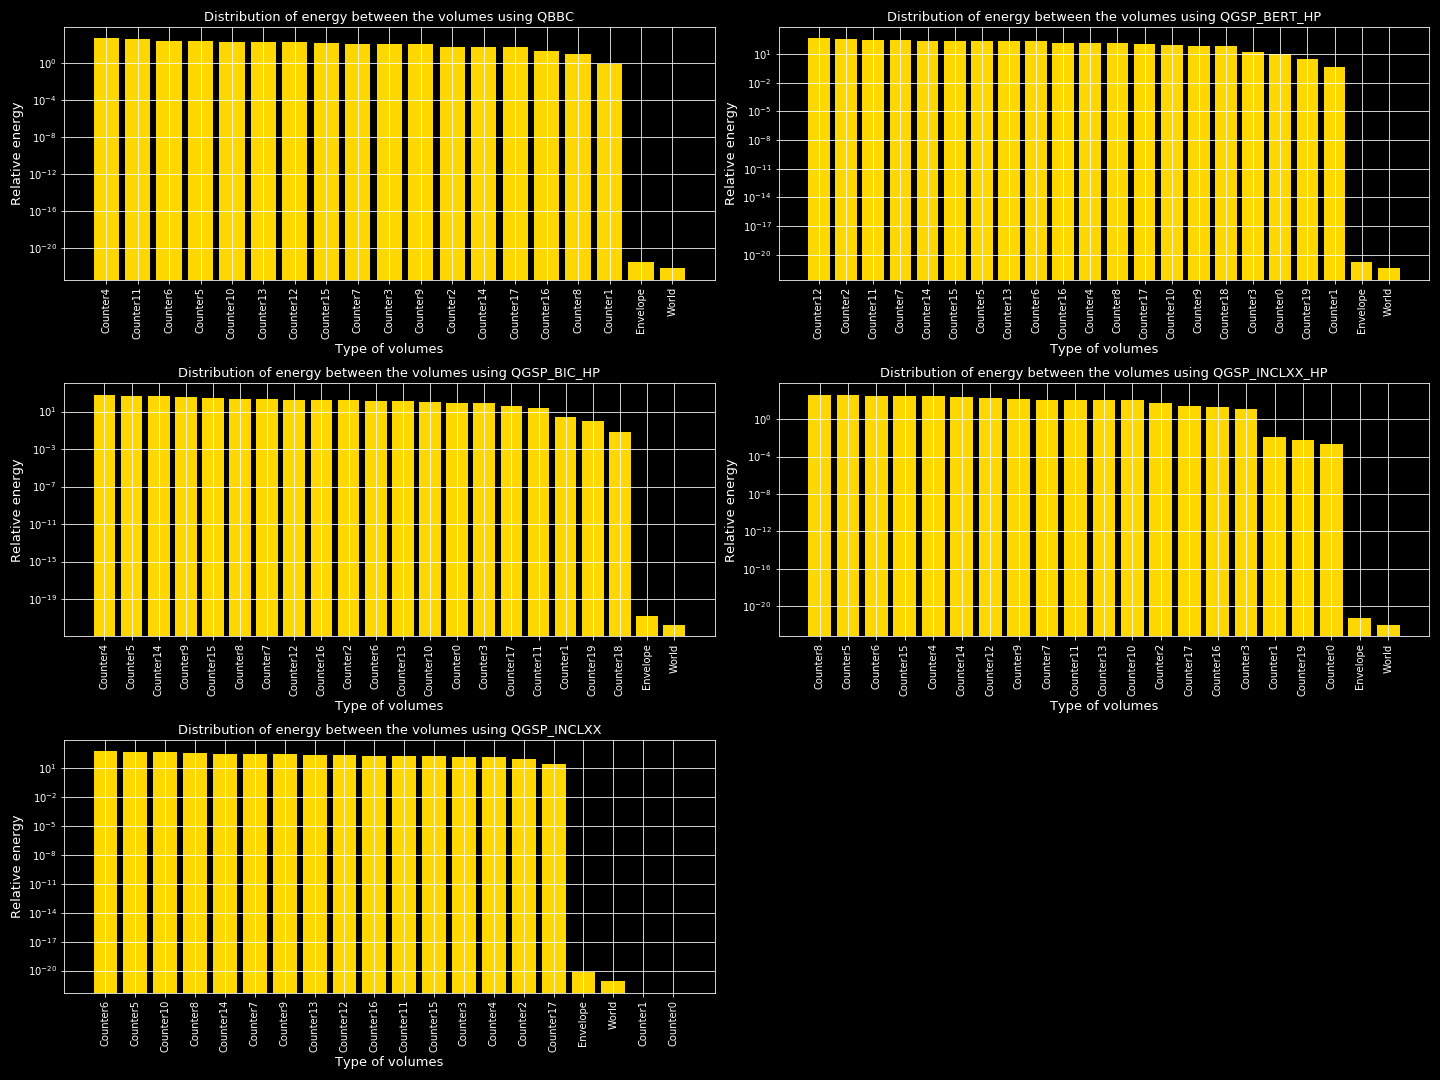
\includegraphics[scale = 0.27]{envol.png}
    \caption{Summing the relative energy distributed among the particles by the volumes they were detected in.}
    \label{fig:my_label}
\end{figure}

\begin{figure}[H]
    \centering
    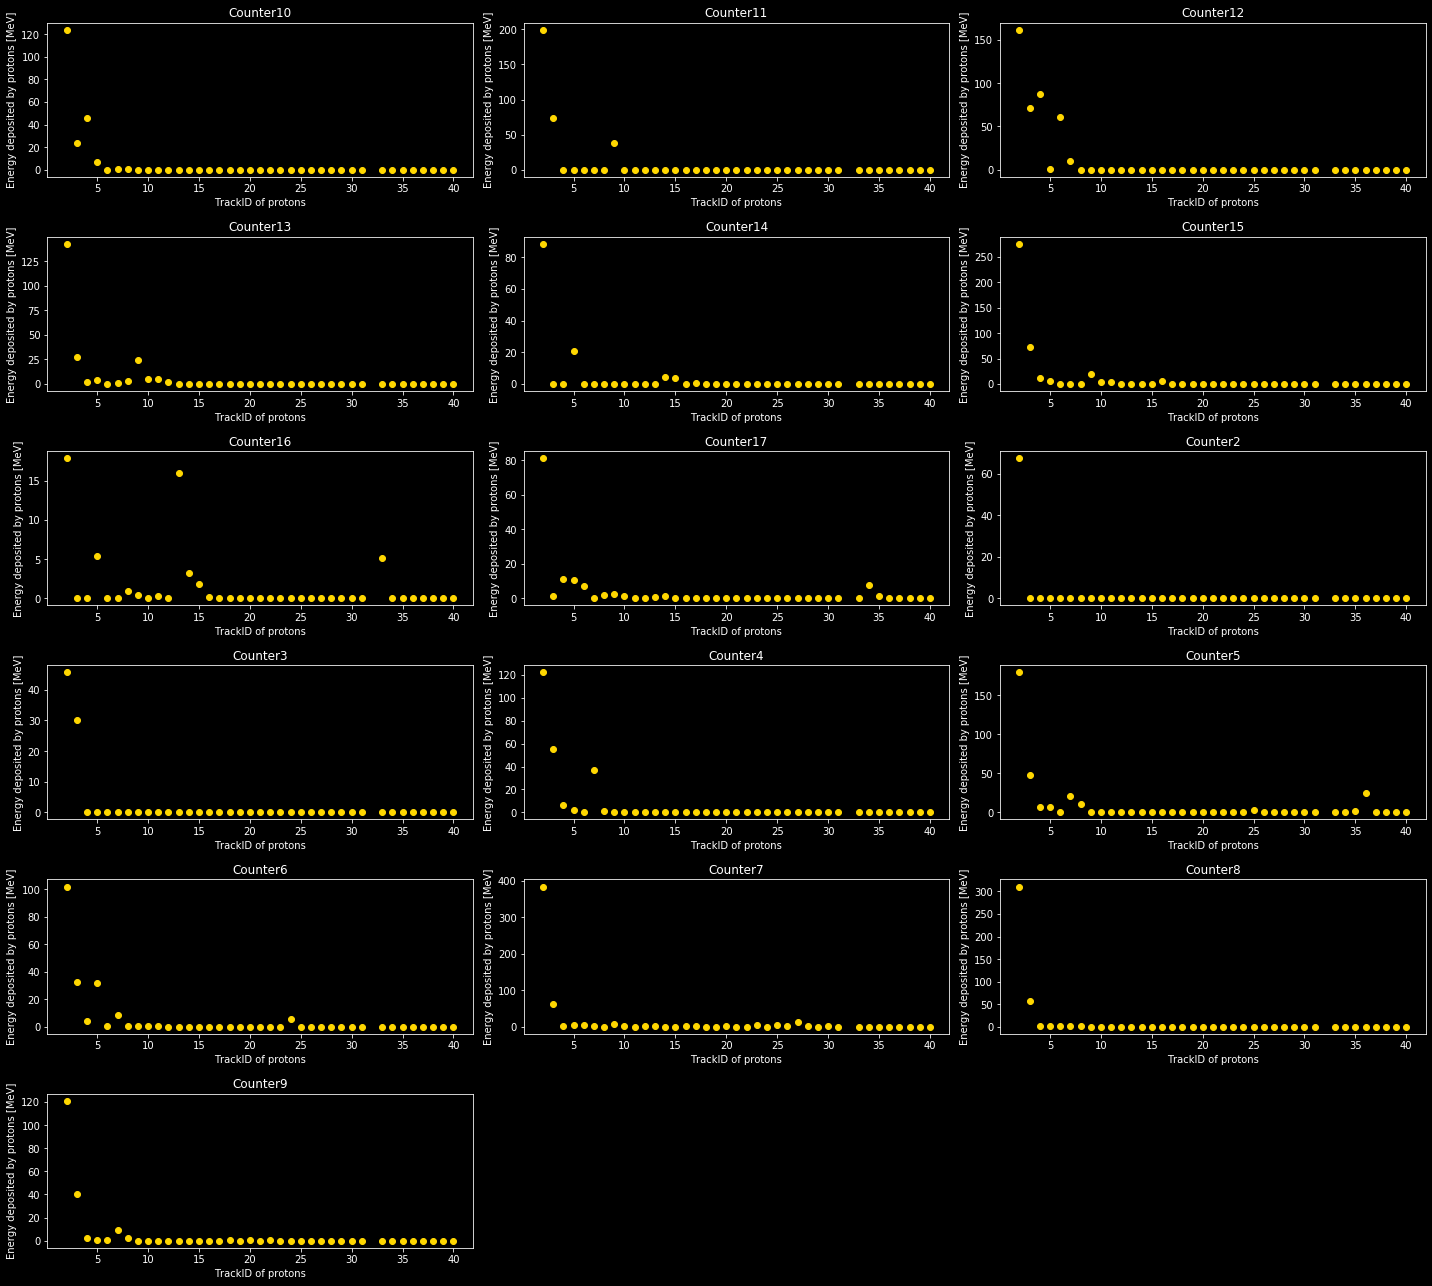
\includegraphics[scale = 0.36]{mat1.png}
    \caption{Energy deposition of protons into the respective volumes during the first run.}
    \label{fig:my_label}
\end{figure}

\begin{figure}[H]
    \centering
    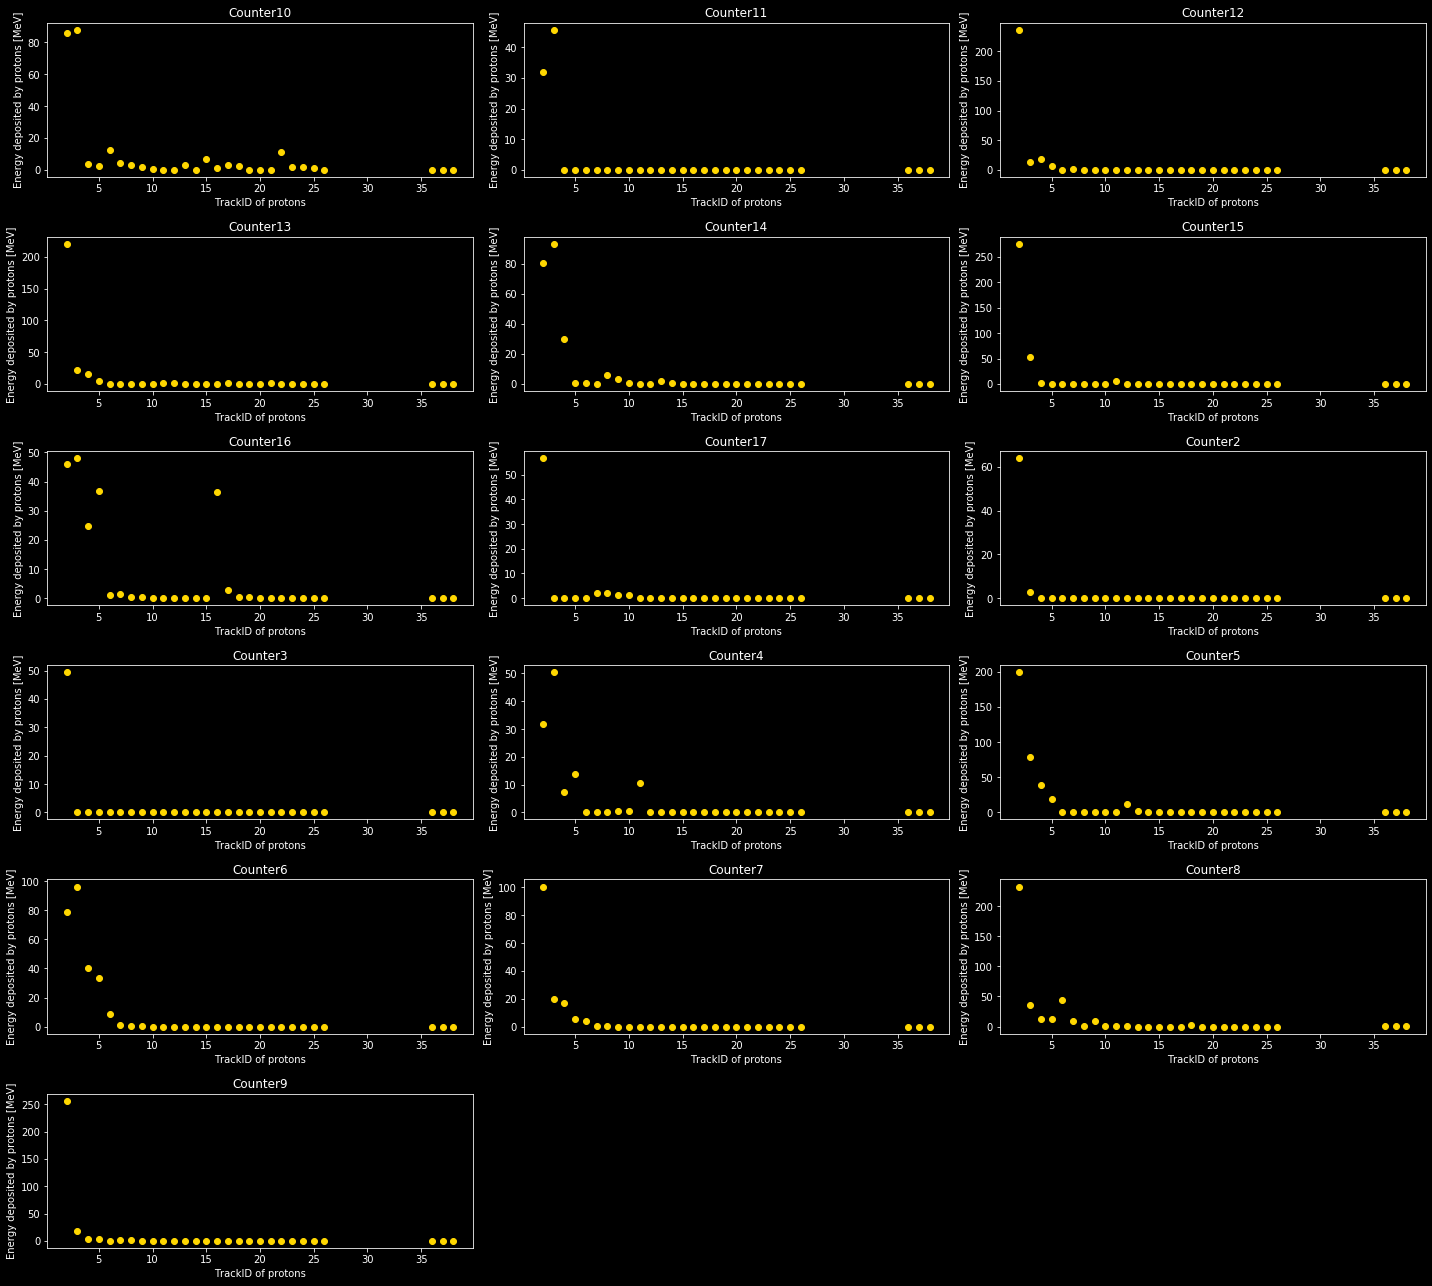
\includegraphics[scale = 0.36]{mat2.png}
    \caption{Energy deposition of protons into the respective volumes during the second run.}
    \label{fig:my_label}
\end{figure}

\begin{figure}[H]
    \centering
    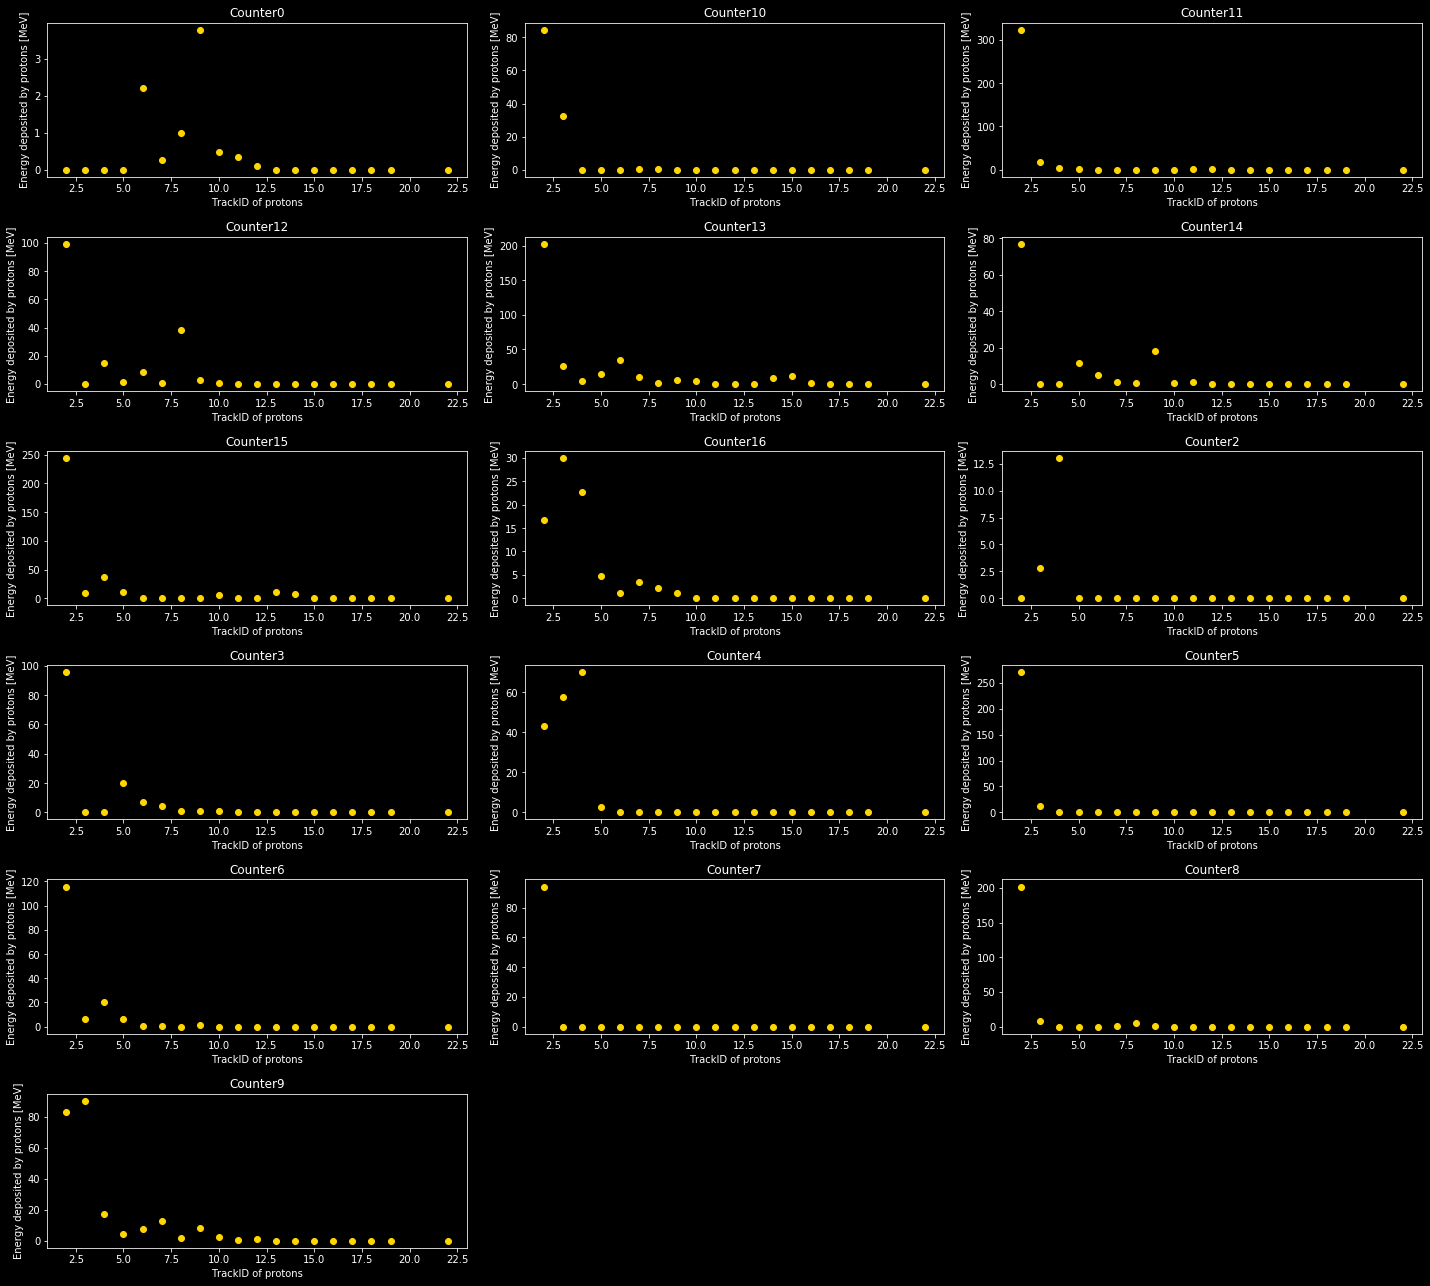
\includegraphics[scale = 0.36]{mat3.png}
    \caption{Energy deposition of protons into the respective volumes during the third run.}
    \label{fig:my_label}
\end{figure}

\begin{figure}[H]
    \centering
    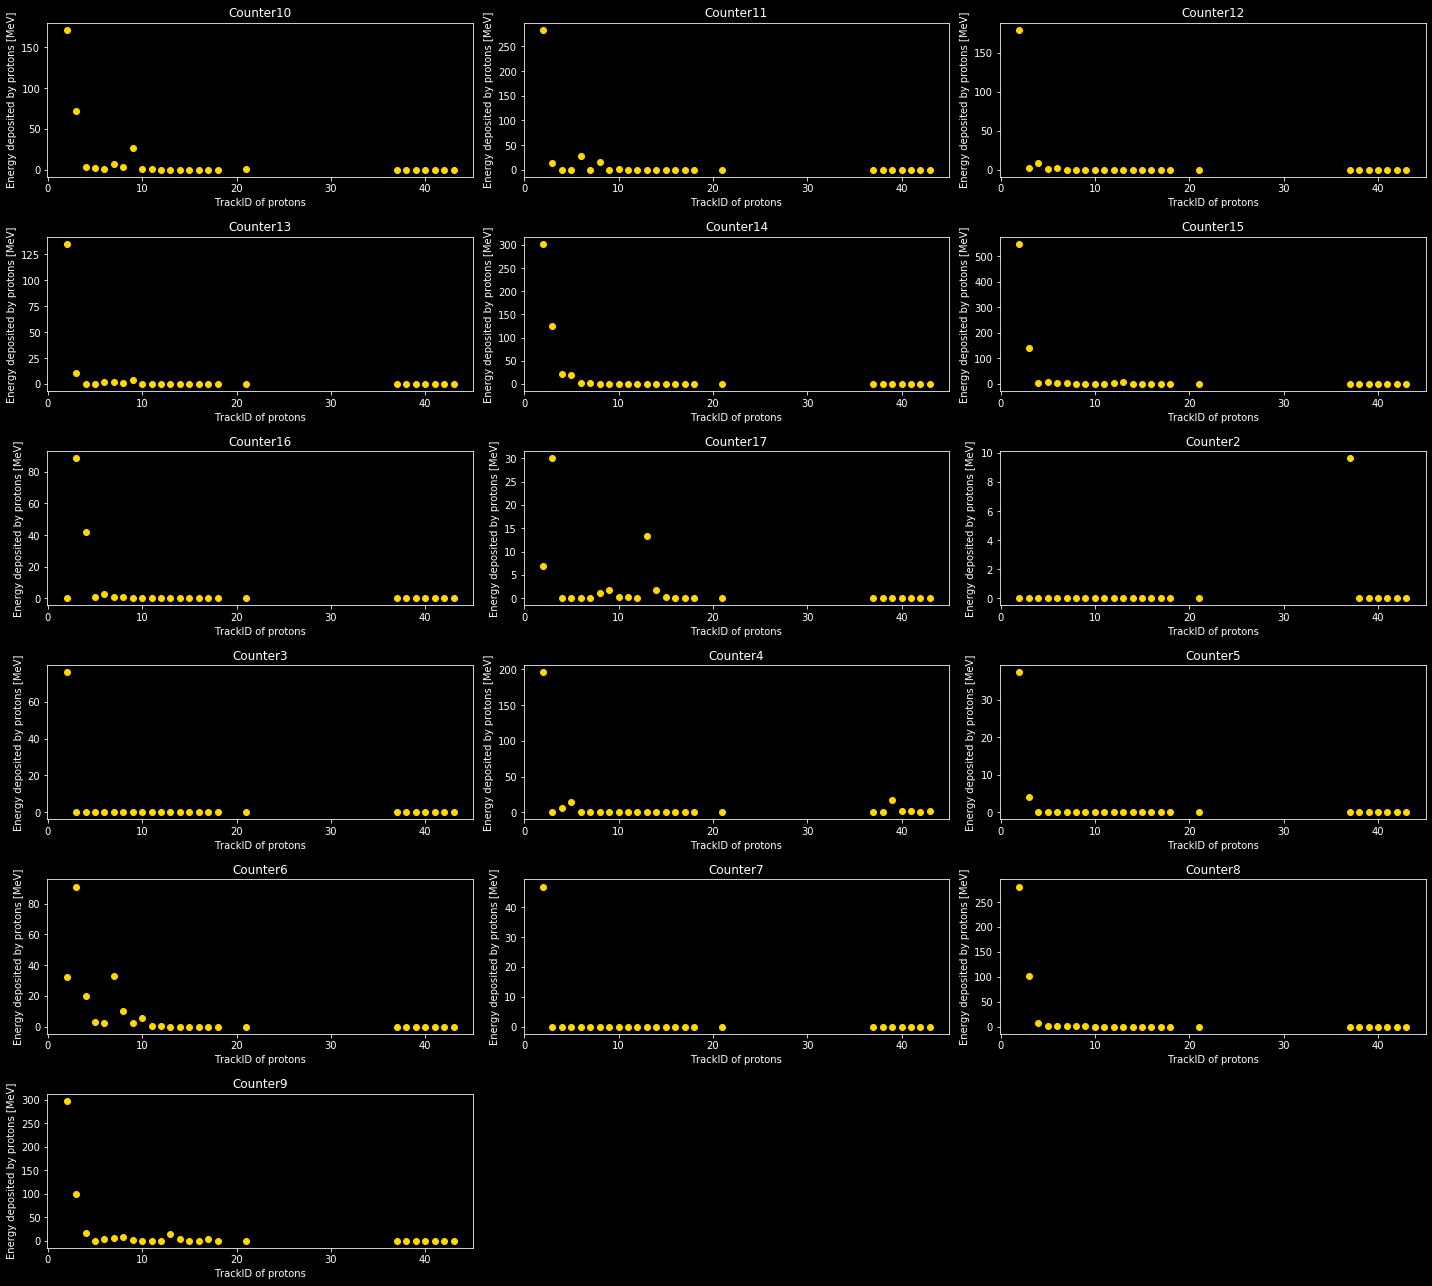
\includegraphics[scale = 0.36]{mat4.png}
    \caption{Energy deposition of protons into the respective volumes during the fourth run.}
    \label{fig:my_label}
\end{figure}

\begin{figure}[H]
    \centering
    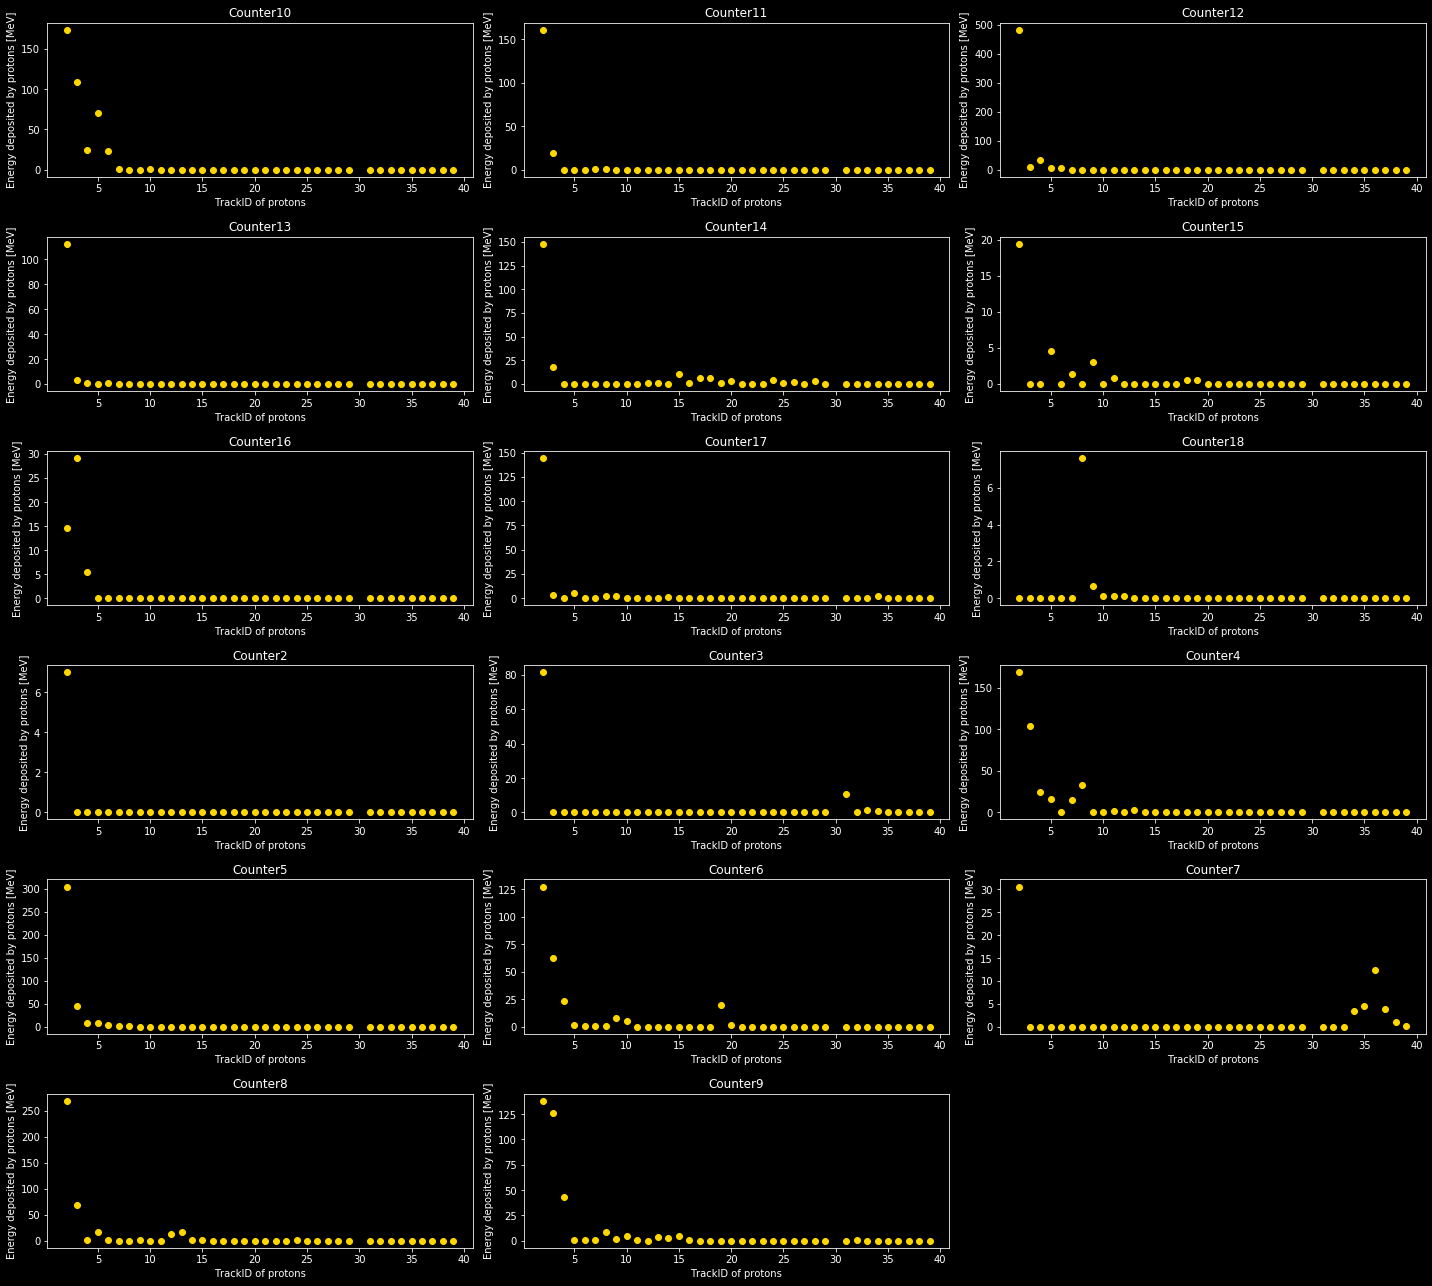
\includegraphics[scale = 0.36]{mat5.png}
    \caption{Energy deposition of protons into the respective volumes during the fifth run.}
    \label{fig:my_label}
\end{figure}

\end{document}
